% results.tex -- DDF-Net terminal validation (drop-in results section).
%
% NOTE: no LaTeX skeleton existed in this repository, so this file is the
% results section and is meant to be \input{} into the paper's main document
% (figures referenced live in ./reports/). Required preamble packages:
%   \usepackage{graphicx, booktabs}
% Adjust the \includegraphics paths if the paper root differs from C:\BMI.

\section{Results: A Real Generative Model Fails the Gate}

To test the gate against a state-of-the-art generative model rather than a
hand-crafted perturbation, we trained the official DDF-Net Stage-1 DDPM
(UNetLidar, 38.93M parameters, $T{=}100$) on subject A01T for 100 epochs and
generated 144 synthetic trials ($72$ left / $72$ right, shape $[144, 22,
1126]$).

\subsection{Covariance structure collapse}

DDF-Net's Stage-1 models each of the 25 channels \emph{independently} (one
$166{\times}600$ image per channel) and concatenates them afterwards, so the
cross-channel spatial covariance is never modelled. Measured against the
calibration class templates (trace-normalized covariance, upper triangle):
real trials achieve cosine similarity $0.9963$ (min $0.9857$, max $0.9993$),
whereas DDF-Net trials collapse to $0.3682$ (min $0.3509$, max $0.3900$) ---
far below the $5$th-percentile acceptance floor of $0.990$.
Figure~\ref{fig:cos-sim} shows the two distributions with the acceptance
window; Figure~\ref{fig:cov} shows the near-diagonal synthetic covariance and
the off-diagonal structure it loses.

\begin{figure}[t]
  \centering
  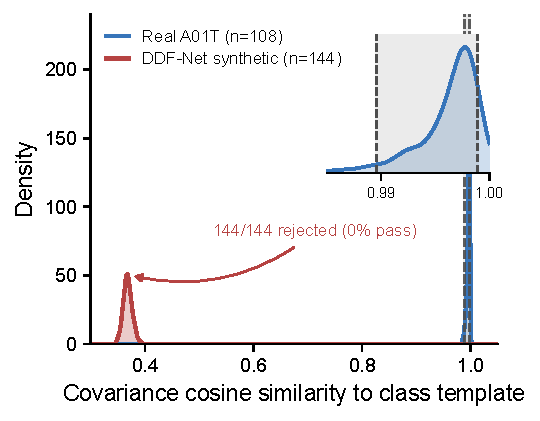
\includegraphics[width=\linewidth]{reports/cos_sim_rejection_distribution.pdf}
  \caption{Covariance cosine-similarity to class template: real A01T vs.\
    144 DDF-Net synthetic trials. All synthetic trials fall outside the
    5--95\% acceptance window.}
  \label{fig:cos-sim}
\end{figure}

\begin{figure}[t]
  \centering
  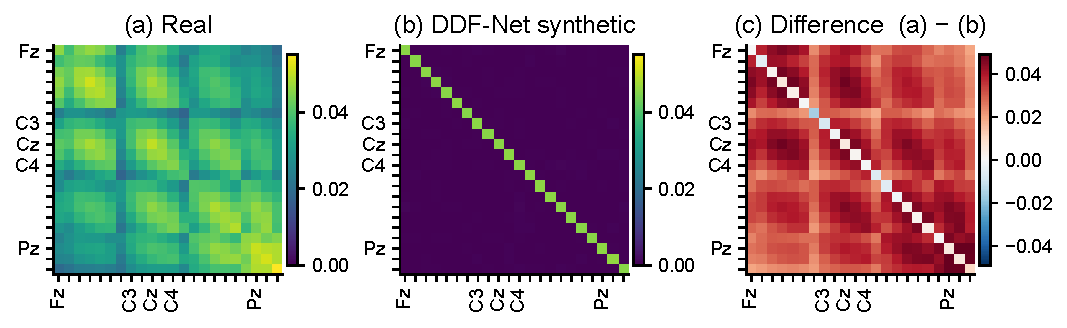
\includegraphics[width=\linewidth]{reports/real_vs_ddf_covariance.pdf}
  \caption{Mean right-hand covariance: (a) real, (b) DDF-Net synthetic,
    (c) difference. Per-channel generation diagonalizes the covariance and
    discards cross-channel structure.}
  \label{fig:cov}
\end{figure}

\subsection{Downstream impact and gate rejection}

\begin{table}[t]
  \centering
  \caption{Downstream CSP+LDA accuracy on the held-out A01T set (36 trials).
    The dual gate rejects all 144 synthetic trials and losslessly restores
    baseline performance.}
  \label{tab:results}
  \begin{tabular}{lcc}
    \toprule
    Condition & Accuracy & Synthetic kept \\
    \midrule
    Baseline        & 0.8333 & --- \\
    Unfiltered      & 0.6667 & 144/144 \\
    Filtered-Cov    & 0.8333 & 0/144 \\
    Filtered-Dual   & 0.8333 & 0/144 \\
    \bottomrule
  \end{tabular}
\end{table}

Table~\ref{tab:results} summarizes the outcome. Injecting the raw synthetic
trials is \emph{harmful}: downstream accuracy drops from $0.8333$ to $0.6667$
($-0.17$), because the collapsed spatial covariance destroys the very
structure CSP consumes. The dual gate passes \textbf{0 of 144} trials (0\%
leakage) and restores accuracy to the baseline $0.8333$ with no loss.

\subsection{Conclusion}

A generative EEG model that fails to model the \emph{joint channel
distribution} produces data that is not merely useless but actively harmful to
downstream decoding. A representation-aligned quality gate is the last line of
defence before deployment.
